\section{Die Sessionverwaltung}

Mehrere verschiedene Benutzer und Benutzerinnen (oder allgemeiner Prinzipale) 
k"onnen gleichzeitig Sitzungen mit dem MyCoRe-Softwaresystem er"offnen. 
W"ahrend einer Sitzung werden in der Regel nicht nur eine sondern mehrere Anfragen bearbeitet. 
Es ist daher sinnvoll, kon\-text\-spe\-zi\-fi\-sche Informationen wie die User ID, die 
gew"unschte Sprache usw. f"ur die Dauer der Sitzung mitzuf"uhren.
Da das MyCoRe-System mit mehreren gleichzeitigen Sitzungen konfrontiert
werden kann, die zudem "uber verschiedene Zugangswege etabliert sein k"onnen
(z.B. Servlets, Kommandozeilenschnittstelle oder Webservices), muss das System
einen allgemein verwendbaren Kontextwechsel erm"oglichen. 

Bei der Bearbeitung einer Anfrage oder Transaktion muss nicht jede einzelne
Methode oder Klasse Kenntnis "uber die Kontextinformationen besitzen.
Daher ist es sinnvoll, die "Ubergabe des Kontextes als Parameter von Methode
zu Methode bzw. von Klasse zu Klasse zu vermeiden.
Eine M"oglichkeit, dies zu bewerkstelligen ist der Einsatz von sog. Thread Singletons oder
thread-local Variablen.
Die Idee dabei ist, den Thread der den Request bearbeitet als Repr"asentation
des Requests selbst anzusehen.
Dazu m"ussen die Kontextinformationen allerdings an den Thread angebunden werden, was
seit Java 1.2 mit Hilfe der Klassen {\bf java.lang.ThreadLocal} bzw. 
{\bf java.lang.InheritableThreadLocal} m"oglich ist.
Jeder Thread hat dabei seine eigene unabh"angig initialisierte Kopie der Variable.
Die set() und get() Methoden der Klasse ThreadLocal setzen bzw. geben die Variable
zur"uck, die zum gerade ausf"uhrenden Thread geh"ort.
Die Klassen der Sessionverwaltung von Mycore sind auf Basis dieser Technologie
implementiert (siehe Abbildung {\ref{fig:Sessionklassen}})

\begin{figure}[h]
  \begin{center}
    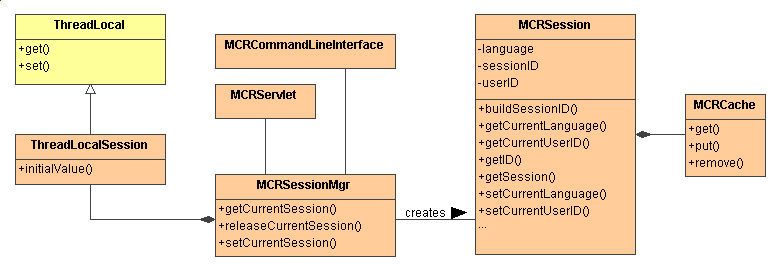
\includegraphics[scale=0.55]{ProgGuide_2Session_classes.jpg}
    \caption{Die Klassen der Sessionverwaltung}
    \label{fig:Sessionklassen}
  \end{center}
\end{figure} 

Klienten der Sessionverwaltung sind alle Klassen, die Kontextinformationen lesen oder
modifizieren wollen, wie zum Beispiel MCRServlet und MCRCommandLineInterface.
Kontextinformationen werden als Instanzen der Klasse MCRSession abgelegt.
Diese Klasse bietet Methoden zum Setzen und Lesen der Informationen, wie z.B.
der User ID der aktuellen Benutzerin, der gew"unschten Sprache usw. 

Die Klasse MCRSession besitzt einen statischen Cache, realisiert durch die Klasse MCRCache.
Bei der Konstruktion einer Instanz von MCRSession wird zun"achst "uber die Methode 
buildSessionID() eine eindeutige ID erzeugt, und diese als Schl"ussel zusammen
mit dem Session-Objekt selbst im Cache abgelegt.
Auf diese Weise hat man "uber die statische Methode getSession() Zugriff auf die zu
einer bestimmten Session ID geh"orende Instanz.

Damit die Instanzen von MCRSession als thread-local Variablen an den aktuellen
Thread angebunden werden k"onnen, werden sie nicht direkt sondern "uber die
statische Methode getCurrentSession() der Klasse MCRSessionMgr erzeugt und sp"ater gelesen.
Beim ersten Aufruf von getCurrentSession() in einem Thread wird "uber die von 
java.lang.Threadlocal erbende, statische innere Klasse ThreadLocalSession gew"ahrleistet, 
dass eine eindeutige Instanz von MCRSession erzeugt und als thread-local Variable
abgelegt wird.
Der Zugriff auf die thread-local Variablen eines Threads kann nur "uber die Klasse
ThreadLocal (bzw. InheritableThreadLocal) erfolgen.
Auf diese Weise ist sichergestellt, dass bei nachfolgenden Aufrufen von getCurrentSession()
genau die zum aktuellen Thread geh"orende Referenz auf die Instanz von MCRSession 
zur"uckgegeben wird. 

Mit der statischen Methode MCRSessionMgr.setCurrentSession() ist es m"oglich, ein 
bereits vorhandenes Session-Objekt explizit als thread-local Variable an den aktuellen
Thread zu binden.
Dies ist z.B. in einer Servlet-Umgebung notwendig, wenn die Kontextinformationen in
einem Session-Objekt "uber eine http-Session mitgef"uhrt werden.
(Aktuelle Servlet Engines verwenden in der Regel zwar Thread-Pools f"ur die Bearbeitung 
der Requests, aber es ist in keiner Weise sicher gestellt, dass aufeinanderfolgende
Requests mit demselben Kontext wieder denselben Thread zugewiesen bekommen.
Daher muss der Kontext in einer http-Session gespeichert werden.)

Die Methode MCRSessionMgr.releaseCurrentSession() sorgt daf"ur, dass das thread-local
Session Objekt eines Threads durch ein neues, leeres Objekt ersetzt wird.
Dies ist in Thread-Pool Umgebungen wichtig, weil es sonst m"oglich bzw. sogar 
wahrscheinlich ist, dass Kontextinformationen an einem Thread angebunden sind, dieser 
Thread aber bei seiner Wiederverwendung in einem ganz anderen Kontext arbeitet.
 
Code-Beispiele zur Verwendung der Sessionverwaltung finden sich in\\ 
org.mycore.frontend.servlets.MCRServlet.doGetPost().
